% =====================================================================
%  Fig. 1b -- ResUNet schematic: flat 2D U-shape + ResBlock inset.
%
%  Channel counts and resolutions correspond to SimpleUNetCond / ResBlock
%  in diffusion/model.py at the manuscript settings base_ch=32,
%  ch_mults=(1,2,4), num_res_blocks=2, on the 180x360 grid. Skip
%  connections are additions, so encoder and decoder share a channel
%  count at every level; it is printed once, on the skip connection.
%  Drawn at final size (17 cm wide).
%
%  Build:  pdflatex -interaction=nonstopmode unet_flat.tex
% =====================================================================
\documentclass[border=4pt]{standalone}
\usepackage[T1]{fontenc}
\usepackage[scaled=0.92]{helvet}
\renewcommand\familydefault{\sfdefault}
\usepackage{amsmath}
\usepackage{bm}
\usepackage{tikz}
\usetikzlibrary{arrows.meta,calc}

% ---- palette (kept close to the superseded figure) -------------------
\definecolor{ResFill}{RGB}{250,224,186}
\definecolor{IOFill}{RGB}{206,236,208}
\definecolor{AddFill}{RGB}{160,214,166}
\definecolor{TFill}{RGB}{214,228,244}
\definecolor{FlowCol}{RGB}{46,105,110}

\begin{document}
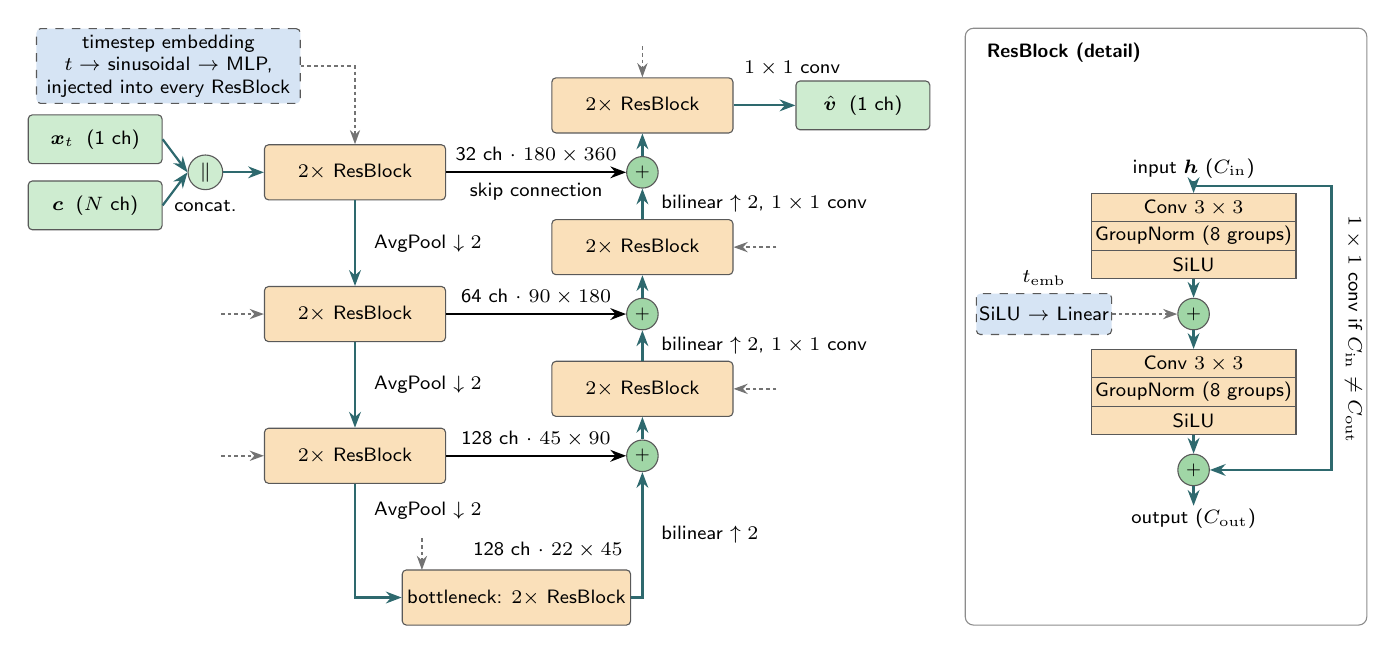
\begin{tikzpicture}[
    x=1cm, y=1cm,
    font=\fontsize{7.5}{9}\selectfont,
    blk/.style={draw=black!65, rounded corners=1.5pt, fill=ResFill,
                minimum width=2.3cm, minimum height=0.70cm,
                align=center, inner sep=1pt},
    bnblk/.style={blk, minimum width=2.9cm},
    io/.style={draw=black!65, rounded corners=1.5pt, fill=IOFill,
               minimum width=1.7cm, minimum height=0.62cm,
               align=center, inner sep=1pt},
    tbox/.style={draw=black!65, dashed, rounded corners=1.5pt, fill=TFill,
                 minimum width=3.35cm, minimum height=0.95cm,
                 align=center, inner sep=1pt},
    ball/.style={draw=black!65, circle, fill=AddFill, inner sep=0pt,
                 minimum size=0.40cm, font=\fontsize{6.5}{7}\selectfont},
    cat/.style={draw=black!65, circle, fill=IOFill, inner sep=0pt,
                minimum size=0.44cm, font=\fontsize{7}{7}\selectfont},
    strip/.style={draw=black!65, fill=ResFill, minimum width=2.6cm,
                  minimum height=0.36cm, inner sep=0.5pt,
                  font=\fontsize{6.8}{7}\selectfont},
    flow/.style={-{Stealth[length=2.0mm,width=1.5mm]}, thick, draw=FlowCol},
    skip/.style={-{Stealth[length=2.0mm,width=1.5mm]}, thick, draw=black},
    temb/.style={-{Stealth[length=1.8mm,width=1.3mm]}, semithick,
                 dashed, dash pattern=on 1.3pt off 1.1pt, draw=black!55},
    lab/.style={anchor=west, font=\fontsize{6.8}{8}\selectfont, inner sep=1pt},
    lvl/.style={font=\fontsize{6.8}{8}\selectfont, inner sep=1pt},
    reslab/.style={font=\fontsize{6.8}{8}\selectfont, inner sep=1pt},
]

% =====================================================================
%  PANEL: the U
% =====================================================================
% rows: encoder blocks / merge points        (pitch \dy = 1.80)
\def\Ra{0}    \def\Rb{-1.80} \def\Rc{-3.60} \def\Rbn{-5.40}
% rows: decoder blocks, \off = 0.85 above their encoder counterpart,
% because the merge happens at the encoder's resolution -- that offset
% is what puts every skip connection on a straight horizontal line
\def\Da{0.85} \def\Db{-0.95} \def\Dc{-2.75}
% columns
\def\Xin{0.85} \def\Xcat{2.25} \def\Xenc{4.15} \def\Xdec{7.80} \def\Xbn{6.20}
% x of the per-level label, centred on the skip run
\def\Xlvl{6.45}

% ---- input ----------------------------------------------------------
\node[io] (xt) at (\Xin, 0.42) {$\bm{x}_t$\; (1 ch)};
\node[io] (cc) at (\Xin,-0.42) {$\bm{c}$\; ($N$ ch)};
\node[cat] (cat) at (\Xcat, 0) {$\|$};
\node[reslab, anchor=north] at (\Xcat,-0.32) {concat.};

% ---- encoder --------------------------------------------------------
\node[blk] (e1) at (\Xenc,\Ra) {$2\times$ ResBlock};
\node[blk] (e2) at (\Xenc,\Rb) {$2\times$ ResBlock};
\node[blk] (e3) at (\Xenc,\Rc) {$2\times$ ResBlock};

% ---- bottleneck -----------------------------------------------------
\node[bnblk] (bn) at (\Xbn,\Rbn) {bottleneck: $2\times$ ResBlock};
\node[lvl] at (6.60,\Rbn+0.60) {128 ch $\cdot$ $22\times45$};

% ---- decoder --------------------------------------------------------
\node[ball] (a1) at (\Xdec,\Ra) {$+$};
\node[ball] (a2) at (\Xdec,\Rb) {$+$};
\node[ball] (a3) at (\Xdec,\Rc) {$+$};
\node[blk] (d1) at (\Xdec,\Da) {$2\times$ ResBlock};
\node[blk] (d2) at (\Xdec,\Db) {$2\times$ ResBlock};
\node[blk] (d3) at (\Xdec,\Dc) {$2\times$ ResBlock};

% ---- output ---------------------------------------------------------
\node[io] (out) at (10.60,\Da) {$\hat{\bm{v}}$\; (1 ch)};
\draw[flow] (d1.east) -- (out.west);
\node[lab] at (9.05,\Da+0.47) {$1\times1$ conv};

% ---- forward flow ---------------------------------------------------
\draw[flow] (xt.east) -- (cat.west);
\draw[flow] (cc.east) -- (cat.west);
\draw[flow] (cat.east) -- (e1.west);

\draw[flow] (e1.south) -- (e2.north);
\draw[flow] (e2.south) -- (e3.north);
\draw[flow] (e3.south) -- (\Xenc,\Rbn) -- (bn.west);

\draw[flow] (bn.east) -- (\Xdec,\Rbn) -- (a3.south);
\draw[flow] (a3.north) -- (d3.south);
\draw[flow] (d3.north) -- (a2.south);
\draw[flow] (a2.north) -- (d2.south);
\draw[flow] (d2.north) -- (a1.south);
\draw[flow] (a1.north) -- (d1.south);

% ---- resampling labels ----------------------------------------------
\node[lab] at (\Xenc+0.20,-0.90) {AvgPool $\downarrow2$};
\node[lab] at (\Xenc+0.20,-2.70) {AvgPool $\downarrow2$};
\node[lab] at (\Xenc+0.20,-4.30) {AvgPool $\downarrow2$};
\node[lab] at (\Xdec+0.20,-4.60) {bilinear $\uparrow2$};
\node[lab] at (\Xdec+0.20,-2.20) {bilinear $\uparrow2$, $1\times1$ conv};
\node[lab] at (\Xdec+0.20,-0.40) {bilinear $\uparrow2$, $1\times1$ conv};

% ---- skip connections, and the one label each level gets -------------
% the merge is an addition, so encoder and decoder share the channel
% count at every level; the number therefore belongs on the skip
\draw[skip] (e1.east) -- (a1.west);
\draw[skip] (e2.east) -- (a2.west);
\draw[skip] (e3.east) -- (a3.west);
\node[lvl] at (\Xlvl,\Ra+0.22) {32 ch $\cdot$ $180\times360$};
\node[lvl] at (\Xlvl,\Rb+0.22) {64 ch $\cdot$ $90\times180$};
\node[lvl] at (\Xlvl,\Rc+0.22) {128 ch $\cdot$ $45\times90$};
\node[lvl] at (\Xlvl,\Ra-0.25) {skip connection};

% ---- timestep embedding ---------------------------------------------
% drawn once, in the free corner above the input, and wired to the first
% ResBlock stack; the short stubs mark the other six
\node[tbox] (temb) at (1.78,1.35) {timestep embedding\\[-1pt]$t \rightarrow$ sinusoidal $\rightarrow$ MLP,\\[-1pt]injected into every ResBlock};
\draw[temb] (temb.east) -- (\Xenc,1.35) -- (e1.north);
\draw[temb] (\Xenc-1.70,\Rb) -- (e2.west);
\draw[temb] (\Xenc-1.70,\Rc) -- (e3.west);
\draw[temb] (\Xdec,\Da+0.75) -- (d1.north);
\draw[temb] (\Xdec+1.70,\Db) -- (d2.east);
\draw[temb] (\Xdec+1.70,\Dc) -- (d3.east);
\draw[temb] (\Xbn-1.20,\Rbn+0.75) -- (\Xbn-1.20,\Rbn+0.35);

% =====================================================================
%  INSET: one ResBlock
% =====================================================================
\def\Xi{14.80}
\draw[draw=black!45, rounded corners=3pt] (11.90,1.83) rectangle (17.00,-5.75);
\node[anchor=north west, font=\fontsize{7.5}{9}\selectfont\bfseries]
    at (12.05,1.77) {ResBlock (detail)};

\node[reslab] (ih) at (\Xi,0.05) {input $\bm{h}$ ($C_\mathrm{in}$)};
\node[strip] (a1s) at (\Xi,-0.45) {Conv $3\times3$};
\node[strip] (a2s) at (\Xi,-0.81) {GroupNorm (8 groups)};
\node[strip] (a3s) at (\Xi,-1.17) {SiLU};
\node[ball] (pt) at (\Xi,-1.80) {$+$};
\node[strip] (b1s) at (\Xi,-2.43) {Conv $3\times3$};
\node[strip] (b2s) at (\Xi,-2.79) {GroupNorm (8 groups)};
\node[strip] (b3s) at (\Xi,-3.15) {SiLU};
\node[ball] (pr) at (\Xi,-3.78) {$+$};
\node[reslab] (oh) at (\Xi,-4.40) {output ($C_\mathrm{out}$)};

\draw[flow] (ih.south) -- (a1s.north);
\draw[flow] (a3s.south) -- (pt.north);
\draw[flow] (pt.south) -- (b1s.north);
\draw[flow] (b3s.south) -- (pr.north);
\draw[flow] (pr.south) -- (oh.north);

% t_emb enters between the two conv-norm-activation pairs
\node[draw=black!65, dashed, rounded corners=1.5pt, fill=TFill,
      minimum width=1.55cm, minimum height=0.52cm, align=center,
      inner sep=1pt, font=\fontsize{6.8}{8}\selectfont] (tp) at (12.90,-1.80)
      {SiLU $\rightarrow$ Linear};
\node[reslab, anchor=south] at (12.90,-1.48) {$t_\mathrm{emb}$};
\draw[temb] (tp.east) -- (pt.west);

% residual branch
\draw[flow] (\Xi,-0.17) -- (16.55,-0.17) -- (16.55,-3.78) -- (pr.east);
\node[reslab, rotate=-90, anchor=south] at (16.68,-2.00)
    {$1\times1$ conv if $C_\mathrm{in}\neq C_\mathrm{out}$};

\end{tikzpicture}
\end{document}
